\documentclass[12pt]{article}
\usepackage{parskip}
\usepackage{amsmath}
\usepackage{pdfpages}
\usepackage{listings}
\usepackage{color}
\usepackage[margin=.6in]{geometry}

\definecolor{dkgreen}{rgb}{0,0.6,0}
\definecolor{gray}{rgb}{0.5,0.5,0.5}
\definecolor{mauve}{rgb}{0.58,0,0.82}

\lstset{frame=tb,
  language=C++,
  aboveskip=3mm,
  belowskip=3mm,
  showstringspaces=false,
  columns=flexible,
  basicstyle={\small\ttfamily},
  numbers=none,
  numberstyle=\tiny\color{gray},
  keywordstyle=\color{blue},
  commentstyle=\color{dkgreen},
  stringstyle=\color{mauve},
  breaklines=true,
  breakatwhitespace=true,
  tabsize=3
}

\begin{document}
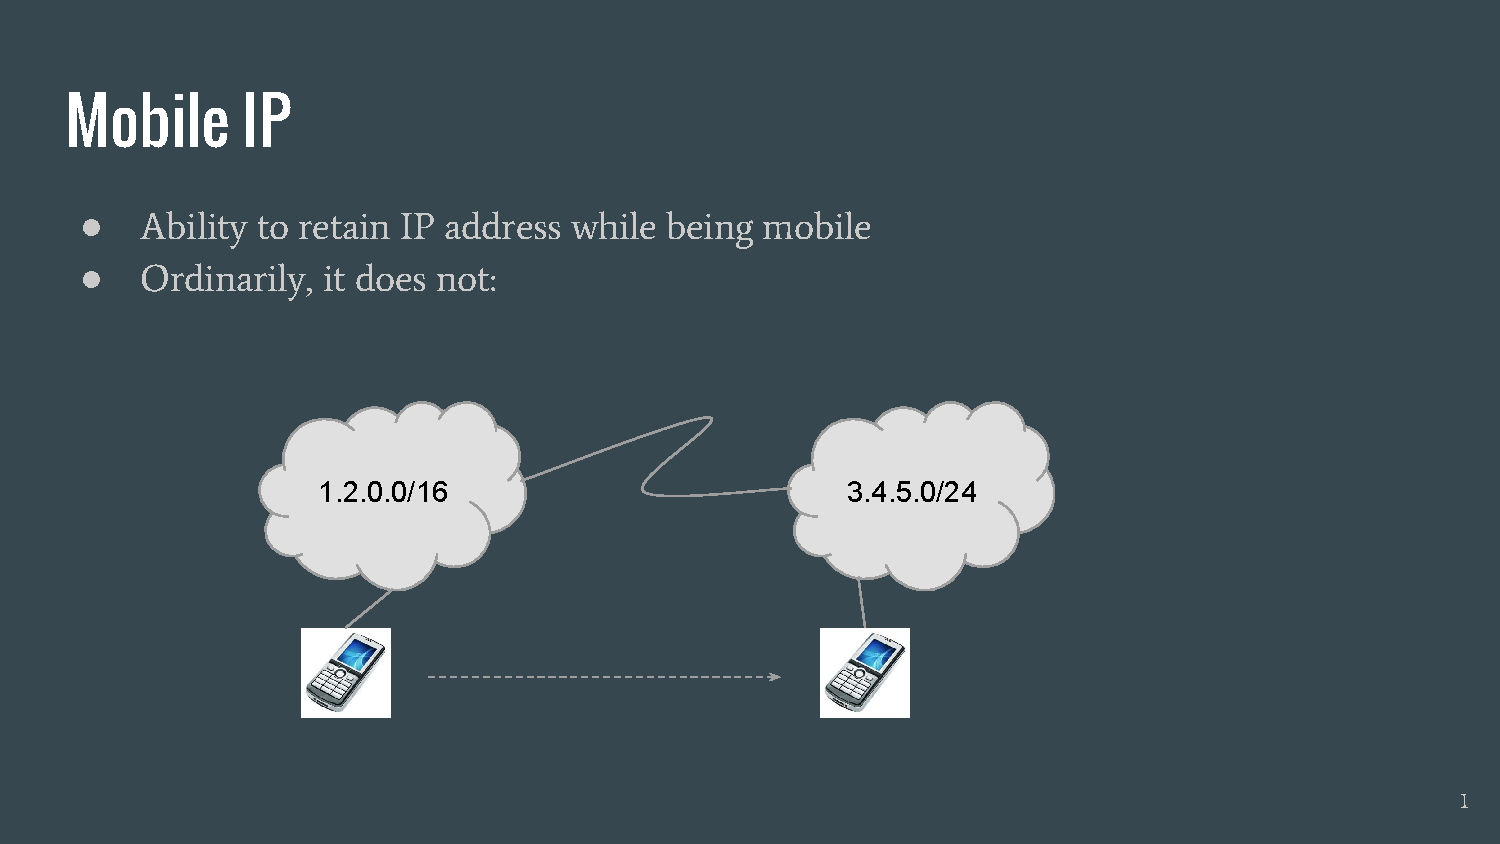
\includepdf[pages=1]{slides.pdf}
We really want to be able to maintain our ipaddress as we move around and jump between networks. Currently no one actually does this, but it'd be cool.

\includepdf[pages=2]{slides.pdf}
Basically we do special routing when an device is on a foreign network.

\includepdf[pages=3]{slides.pdf}
The RFC for mobile routing makes some assumptions. The big one is the assumption that all routing is destination address based. This is not necissarily true because people will often put values in and use those to take short cuts to speed up internet.

\includepdf[pages=4]{slides.pdf}
\includepdf[pages=5]{slides.pdf}
\includepdf[pages=6]{slides.pdf}
Each device actually get two addresses, the one it has on the home address and the care of address from the foreign network. When the mobile device joins a foreign network it notifies the home agent what its new care of address. The home agent passes packets from the device to corresponding nodes, called \textbf{tunneling}.

\includepdf[pages=7]{slides.pdf}
A common form of tunneling is encapsulation. This is basically just appending another header with new data onto the packet.

\includepdf[pages=8]{slides.pdf}
While a mobile address is on a foreign address its legitimate address is its home address, but it can send out a packet saying that the source address is its care of address.

\includepdf[pages=9]{slides.pdf}
Mobile routing adds a bunch of hops which can slow things down. To optimize this the mobile node passes a bunch of data around to try to notify everyone (its a stupid complicated thing, don't bother learning too much about it).

\includepdf[pages=10]{slides.pdf}
\includepdf[pages=11]{slides.pdf}
\includepdf[pages=12]{slides.pdf}
There are two models discussed for problem 1. Strong hosts only look for packets going to a specific interface, and weak hosts look for a packet going to any interface. With weak host models. 

\includepdf[pages=13]{slides.pdf}
A host B might want to address a packet to the public interface of host A (not to its internal ethernet address) if it is using a domain name service to find it. You could also have an application that only binds itself to the public ipaddress of A. Problems can occur if you mix strong and weak hosts. For instance a weak host cannot sent to a strong host and attackers can spoof a packet to look like it originates from the local network (like its id is 2030.113.2) then the weak host will think its trusted and forward it making it seem more trustworthy than it actually is.

Ipaddress spoofing is when someone lies about their source address. 

\includepdf[pages=13]{slides.pdf}
\includepdf[pages=14]{slides.pdf}
\includepdf[pages=15]{slides.pdf}
What address do we use as the source address when we send something? Basically we just come up with some rules to decide. This is a common problem for load balancing.


















\end{document}